\documentclass[a4paper]{article}
\usepackage{graphicx}
\graphicspath{/home/angelo/Documents/Uni/Courses/Advanced Statistics and programming/Assignments/assignment2/} 
\usepackage{mathtools}
\usepackage[a4paper, total={5in, 6.5in}]{geometry}
\usepackage{color}
\usepackage{tikz}
\usepackage{lipsum}
\usepackage{geometry}
\geometry{a4paper, left=2.5cm, top=2.5cm, bottom=2.5cm, right=2.5cm}
\usepackage{changepage}
\usepackage{booktabs}
\usepackage[font=small]{caption}
\DeclareCaptionFormat{mycaptionfont}{\fontsize{12}{13}\selectfont#1#2#3}
\usepackage{threeparttable}
\usepackage{ntheorem}
\usepackage{caption}
\usepackage{wrapfig,lipsum,booktabs}
\usepackage{listings}
\usepackage{pdflscape}
\captionsetup{format=mycaptionfont}
\usepackage{subcaption}
\theoremseparator{:}
\usepackage{lscape}
\usepackage{rotating}
\usepackage[utf8]{inputenc}
\newtheorem{hyp}{Hypothesis}
\usetikzlibrary{shapes,decorations,arrows,calc,arrows.meta,fit,positioning}
\tikzset{
    -Latex,auto,node distance =1 cm and 1 cm,semithick,
    state/.style ={ellipse, draw, minimum width = 0.7 cm},
    point/.style = {circle, draw, inner sep=0.04cm,fill,node contents={}},
    bidirected/.style={Latex-Latex,dashed},
    el/.style = {inner sep=2pt, align=left, sloped}
}





\begin{document}

\title{ASAP Assignment 2}
\author{Angelo Barisano; 508903 }
\date{September 23rd, 2022}
\maketitle

\newpage
\section{Difference in Difference}






\subsection{Task 1: Derive Diff-In-Diff Coefficients}

$(1-1) \ {y_{it}} = \beta_{0} + \beta_{1} D_i + \beta_{2} T_t+ \beta_{3} D_i T_t + \epsilon_{it}$



Considering the canonical difference-in-difference equation expressed in regression form (1-1), the individaul outcome of ${y_{it}}$ is defined by five terms:

\begin{enumerate}
	\item $\beta_{0}$; constant - will be cancelled out in later part
	\item $\beta_{1} D_i$; treatment indicator - whether the subject is treated or not represented by either (D= 1$ | $D = 0)
	\item $\beta_{2} T_t$; independent of the subject, the "event study" contains pre- and post-test measurements indicator for each subject
	\item $\beta_{3} D_i T_t$; the interaction effect of the treatment indicator and the time indicator displays the assumed effect of the change from pre to post test in $T_t$ for an individual in the treatment or control - in case of treatment, this term falls out as the general assumtion of diff-in-diff pertains to the control being the same as the treatment. 
	\item $\epsilon_{it}$; contains the disturbances
\end{enumerate}


The terms in 2, 3, \& 4 are relevant in describing the potential outcome assumption in difference in difference analysis. Difference in difference suggests that we compare the difference between treatment and control before and after the treatment introduction (t = 0), shown as:



$
(1-2) \ [E(y_{T=1} | D=1) - E(y_{T=0} | D=1)] - [E(y_{T=1} | D=0) - E(y_{T=0} | D=0)]
$


Subsequetnly, the four outcomes described in (1-2) yield the following outcomes:

\begin{itemize}
\item $E = (y_{T=1} | D=1)$; Becasue we are observing the outcome for the post-(treatment) test for treatment group, this yields $\beta_{0}$, $\beta_{1}$, $\beta_{2}$, $\beta_{3}$ 
\item $E = (y_{T=0} | D=1)$; Because we are observing the outcome of the pre-(intervention) test for the treatment, this will yield $\beta_{0}$, $\beta_{1}$
\item $E = (y_{T=1} | D=0)$; Becasue we are observing the outcome for the post-(treatment) test for the control group, this yields $\beta_{0}$, $\beta_{2}$ 
\item $E = (y_{T=0} | D=0)$; Because we are observing the outcome of the pre-(intervention) test for the control, this will yield $\beta_{0}$
\end{itemize}

Note that the disturbance term is left out as it is assumed to be independent of the treatment selection etc.; as such we will ignore it here. 
Additionally, the constant is present in all four outcomes; thus, it also cncels out in the following equation. This originates from the assumption that the covariates measurments in pre and post test yield the same results for both treatment and control subjects. Equivalently, by substitution the aforementioned outcomes into (1-2), the following results can be deduced:

\

$
(1-3) \ E(y_{it}) =  [E(y_{T=1} | D=1) - E(y_{T=0} | D=1)] - [E(y_{T=1} | D=0) - E(y_{T=0} | D=0)]
$

\

$
(=) \ E(y_{it}) = [(\beta_{1} + \beta_{2} + \beta_{3}) - (\beta_{1})] - [(\beta_{2})]
$

\

$
(=) \ E(y_{it}) = (\beta_{2} + \beta_{3}) - \beta_{2} = \beta_{3}
$

\



\textbf{NOte possibly delete duplicates}



Important: we canot identify the monthrs; so If they become mothers at some point, we will assume that these are taken out!




\subsection{Task 2: Provice Graphical "evidence" for the presence of the DiD effect}

\begin{wrapfigure}{L}{9cm}
\centering
\begin{subfigure}[b]{0.5\textwidth}
    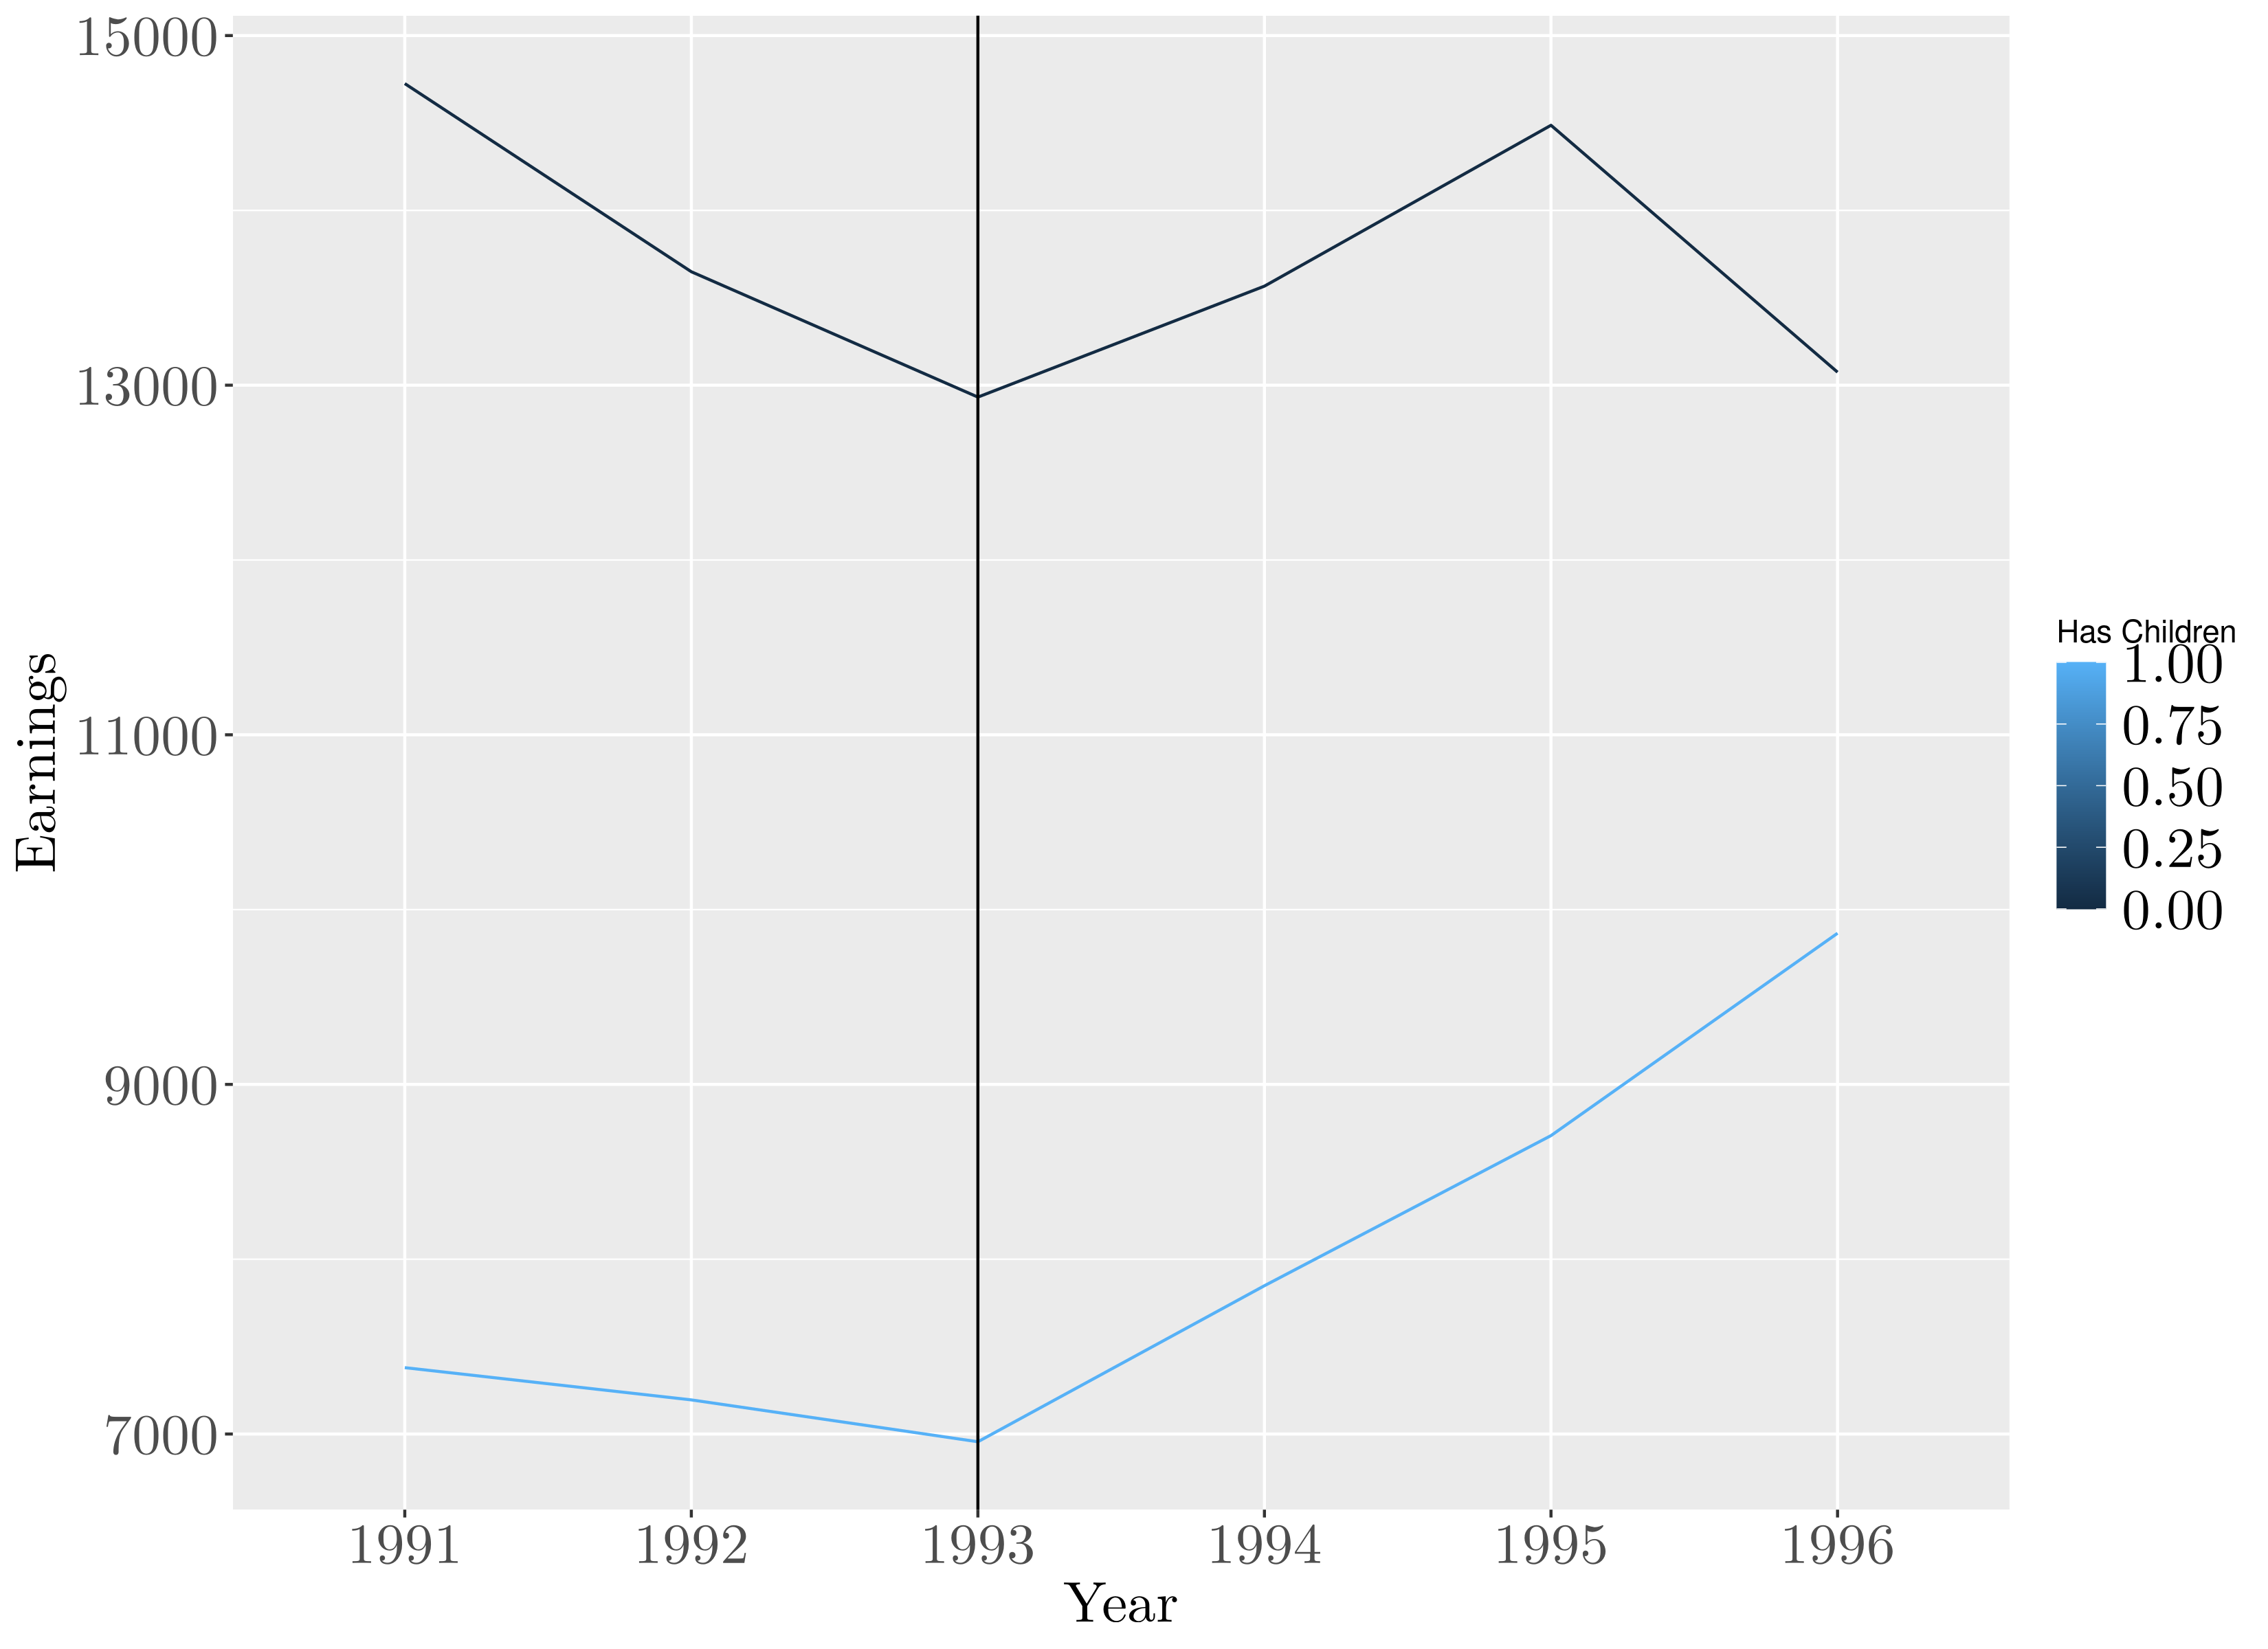
\includegraphics[width=.95\linewidth]{"/home/angelo/Documents/Uni/Courses/Advanced Statistics and programming/Assignments/assignment2/Graphics/task2_earn_did.png"} 
   \caption{Annual Earnings by Females with(out) Children}
   \label{fig:Ng2}
\end{subfigure}

\begin{subfigure}[b]{0.5\textwidth}
    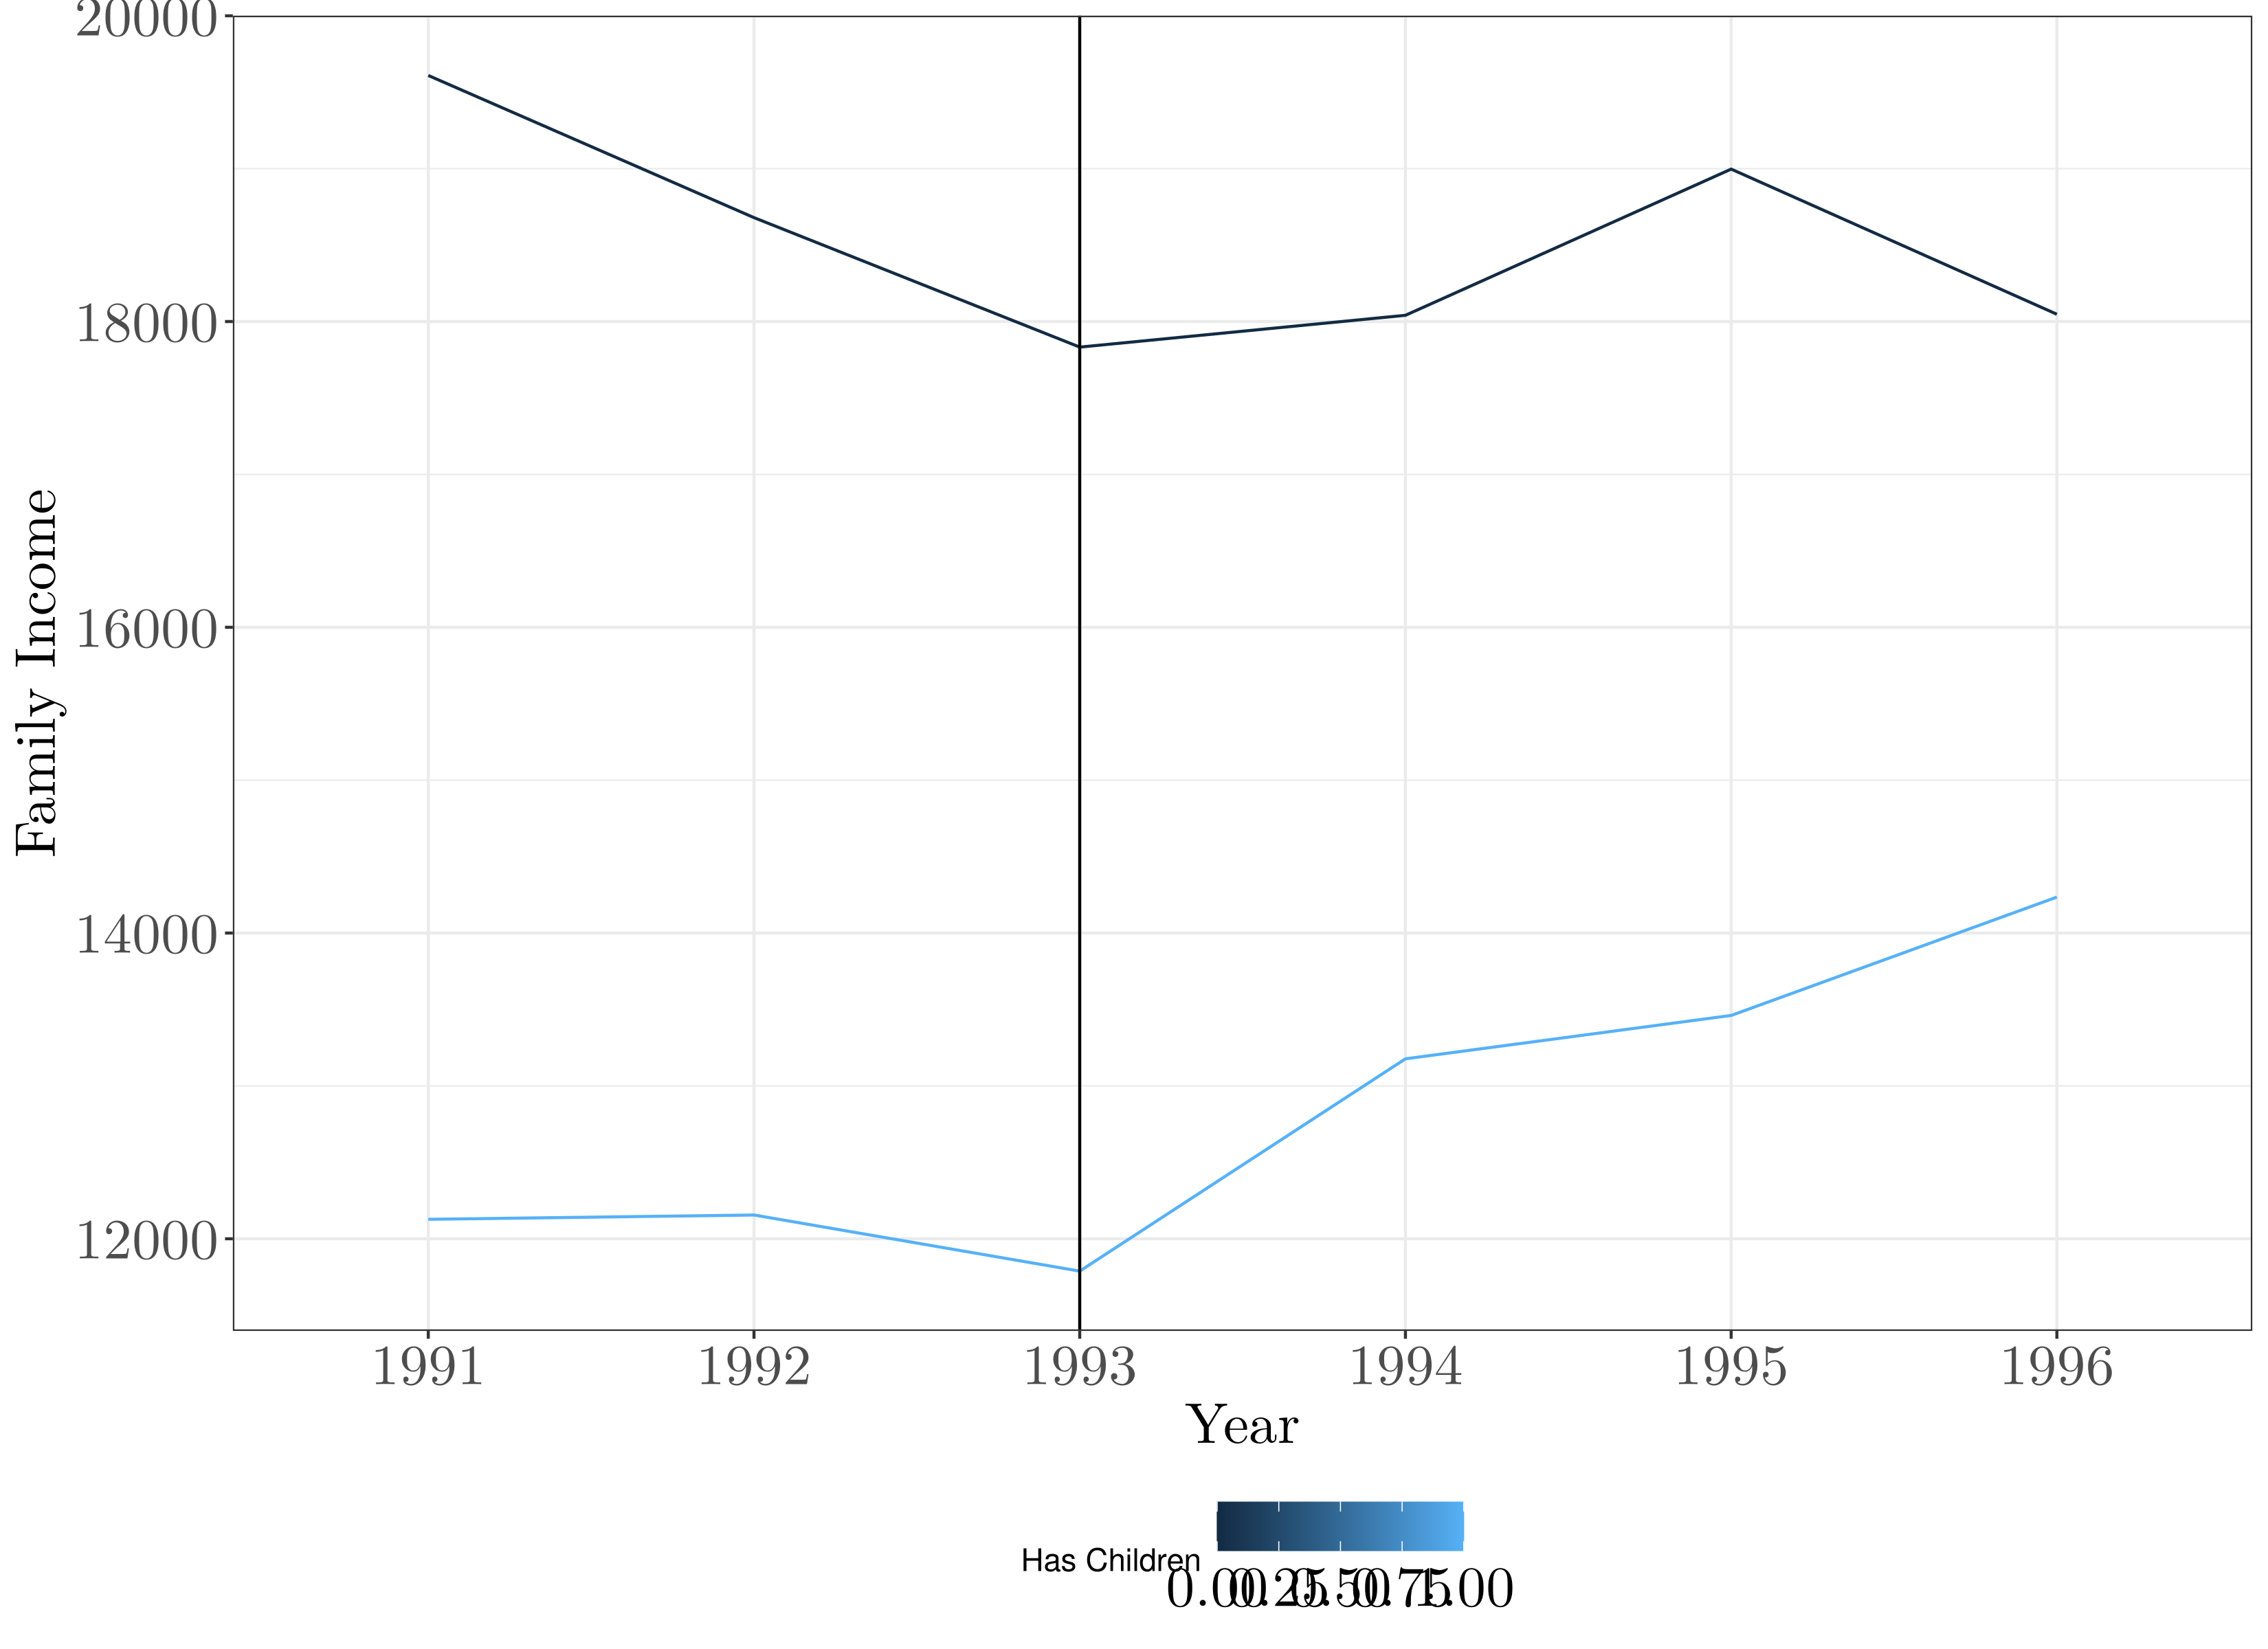
\includegraphics[width=.95\linewidth]{"/home/angelo/Documents/Uni/Courses/Advanced Statistics and programming/Assignments/assignment2/Graphics/task2_finc_did.png"} 
   \caption{Family Earnings Earnings by Females with(out) Children}
   \label{fig:Ng2}
\end{subfigure}

\begin{subfigure}[b]{0.5\textwidth}
    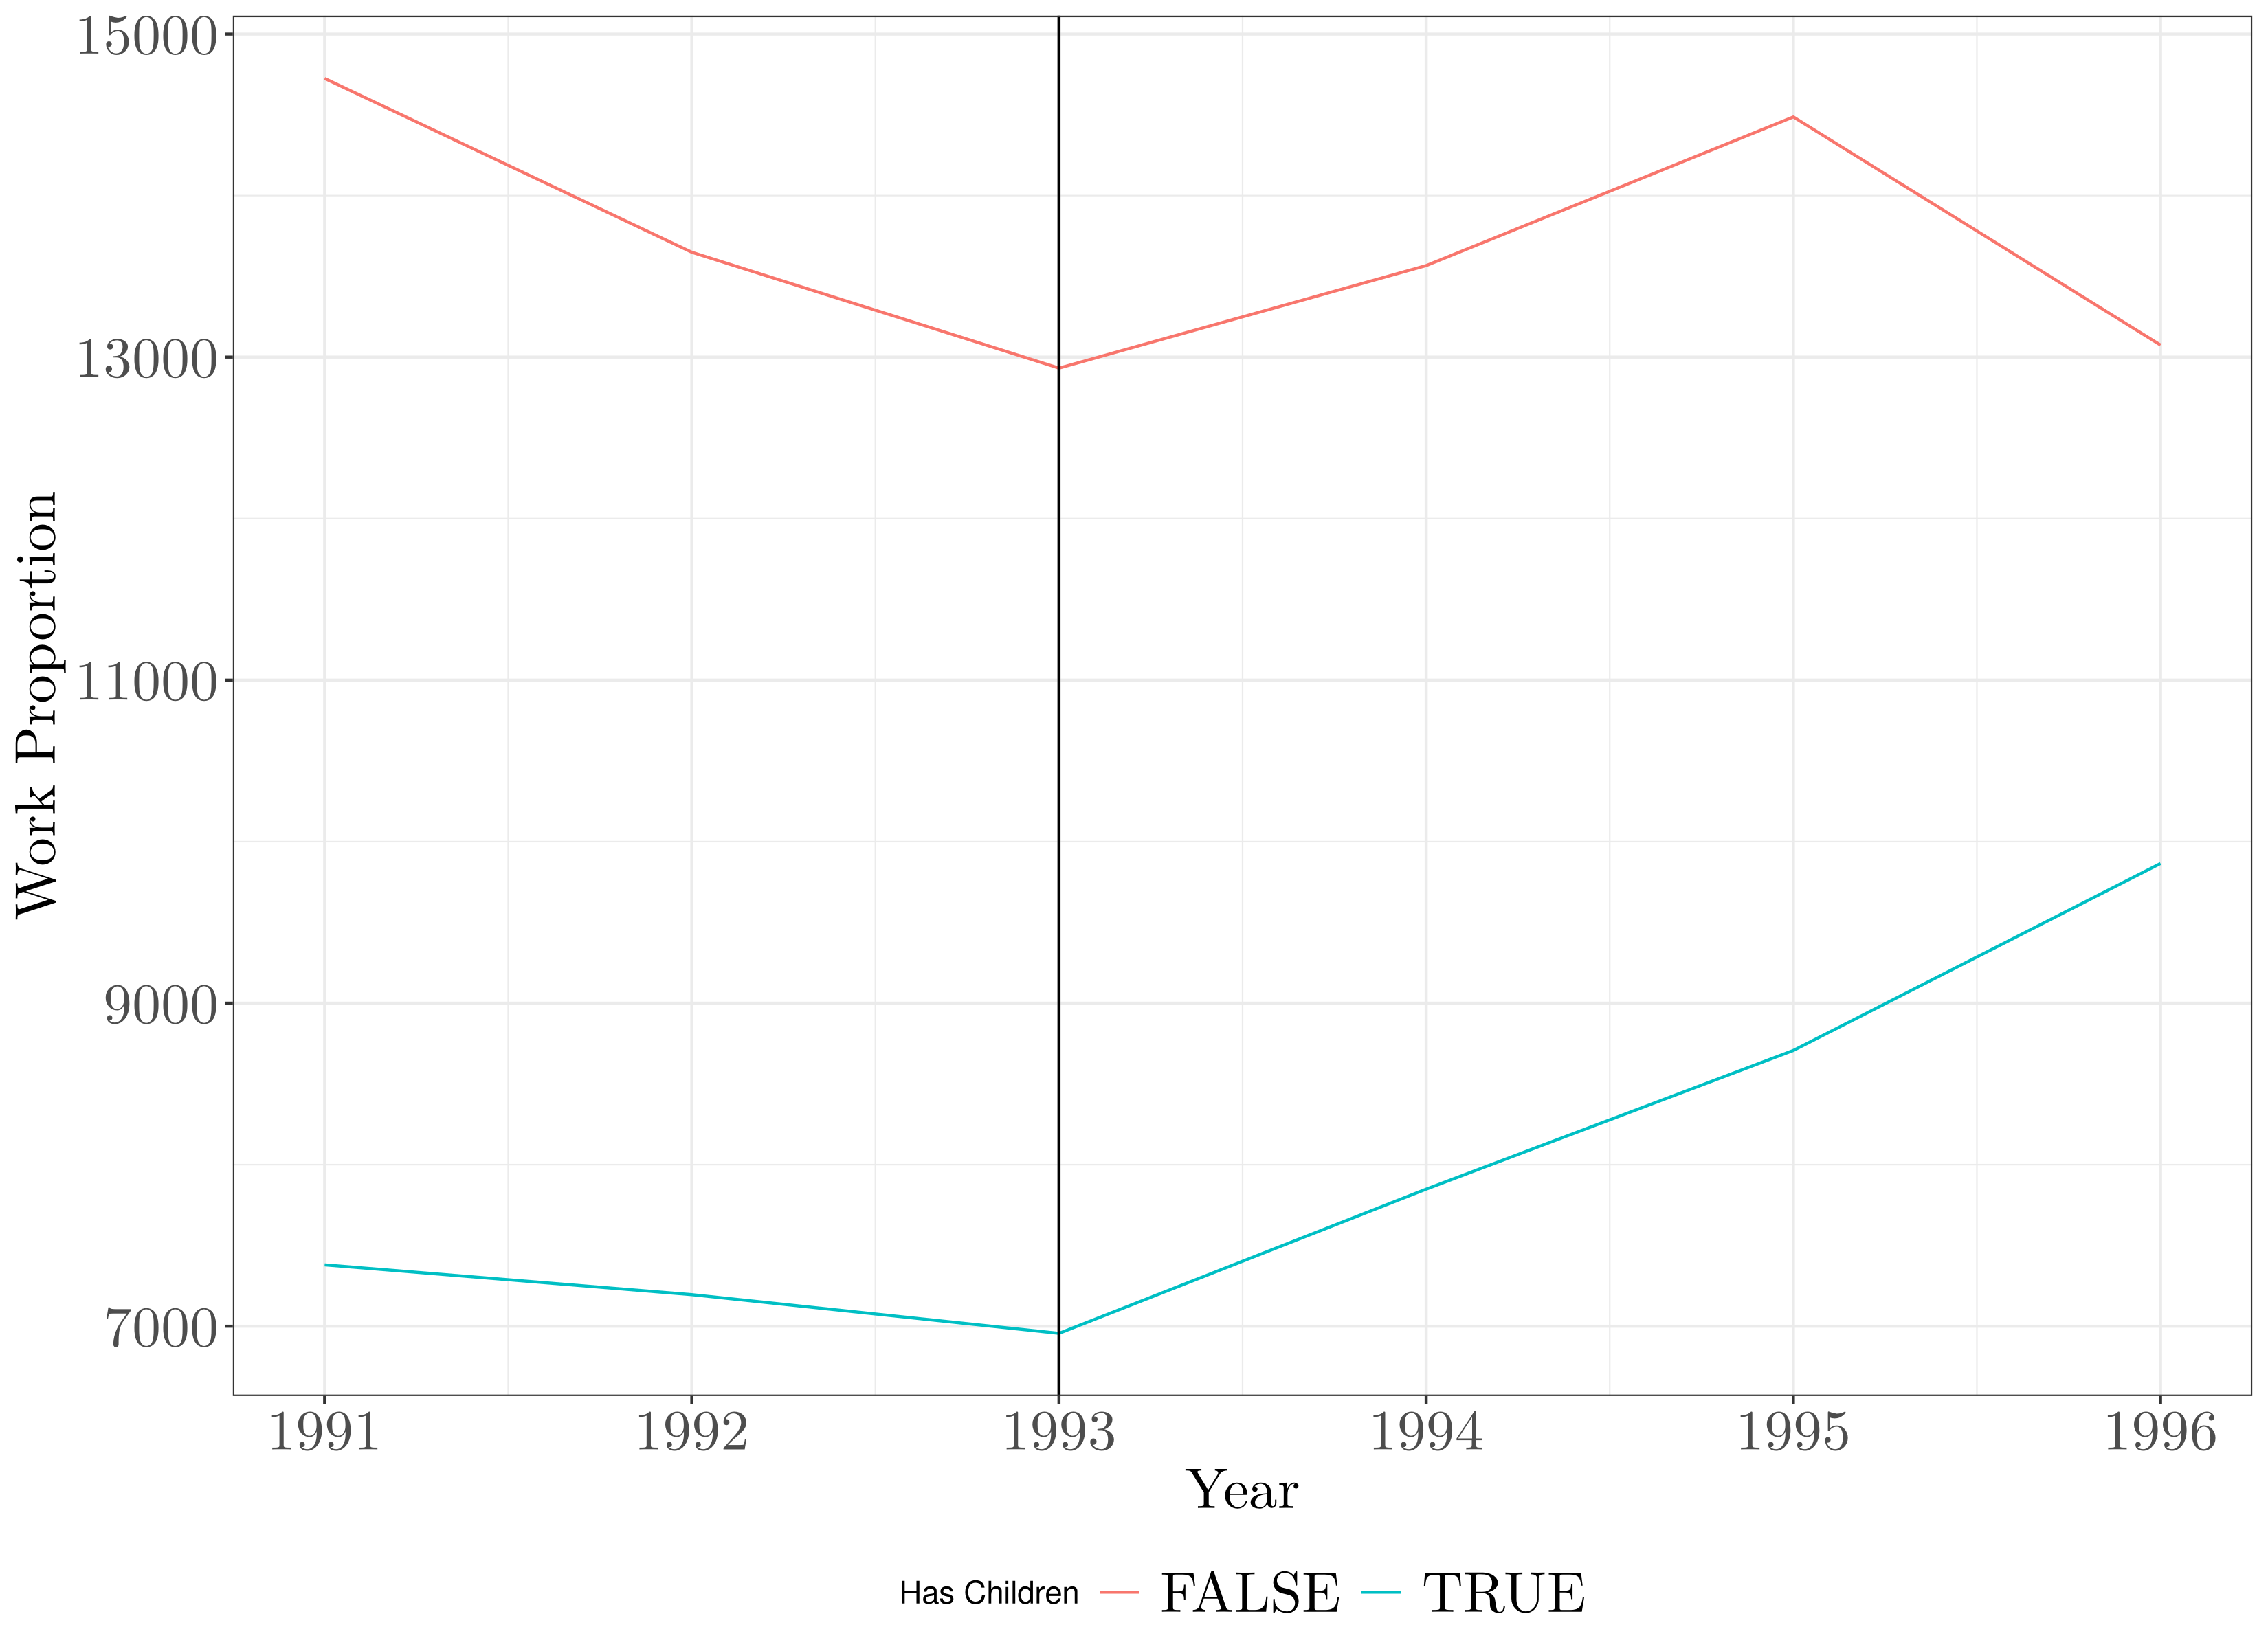
\includegraphics[width=.95\linewidth]{"/home/angelo/Documents/Uni/Courses/Advanced Statistics and programming/Assignments/assignment2/Graphics/task2_work_did.png"}  
   \caption{Work Participation by Females with(out) Children}
   \label{fig:Ng2}
\end{subfigure}
\captionsetup{justification=centering}
\caption{Pre-Post Intervention of EICT Credit for Women with(out) Children}
\end{wrapfigure}

Figure 1 displays the outcomes for both treatment and control group for earnings (earn), family income (finc), and work-participation indicator (work) over the period form 1991 to 1996. THe treatment in this case is defined as a binary state of Females with children (one or many) (D = 1) and females without children (D = 0).\footnote{I do refer to females/ males as the study subject in question}. The tax credit (EITC) is assumed to be introduced on the 1st of January 1993.\footnote{see canvas discussion board}
\indent Figure 1 a) displays the development of earnings and the introduction of the EITC is marked by the vertical line (as in the other graphics). Females without children earned considerably more on average than females with children, starting out at slightly less than \$14800 and dropping to \$13000 at its lowest. Overall, both groups displayed a downward trend before 1993. After 1993, the supposed introduction of the EITC, both groups experienced an increase in earnings; However, the childless group did not display a continous increase in earnings when compared to females with children, which displayed a continous increase of earnings after the introduction. This might suggest that the introduction of the  EITC is associated to the average earnings of women with children but not for women without children.
\indent Figure 1 b) shows the same features as the plot before but the outcome is now Family Income. Overall, the point of origin general trend is similar for both groups as in Figure 1 a); it may be noted that the trend for females with child is less pronounced than in a). Thus, the conclusion is the same as in a): an overall positive trend is displayed for females with children, while childless females do not improve considerably during the post period. 
\indent Figure 1 c) displays workparticipation of females with and without children.Again, childless women start out higher at around 54\% workparticipation vs 46\% workparticipation for women with children. Moreover, the trends are somewhat comparable to the two preceeding graphics, as females with children display an increase to 50.3\% (and then a slight drop in the following year), while childless women tend to decrease. Thus, on average during the post treatment period, we see a substantial increase for women with children in workparticipation.






\begin{enumerate}
   \item Describe each picture and what you can see; but also note that this is based on averages and not statistically true
   \item IMPORTANT: you should look at the grading grid of the previous assignment to see what their requirements are for these
\end{enumerate}



\subsection{Task 3: Summary Statistics for data}
The dataset is not balanced and we cannot assure that it is fixed. Nonetheless, for the purpose of this exercise, it is assumed that it is balanced and fixed. The data contains yearly records from 1991 to 1996; the reported values per variable are thus averages over all six years. A total of 13746 records were made, split by year into 2610, 2449, 2342, 2255, and 2085 observations respectively. Of the total 13746 observations, 7819 have one or more children, and 5927 has no children.\footnote{additional summary statistics can be found for women with and without children in Appendix 4.1}. Of the relevant outcome variables (earnings, family income, work participation), the average family income was \$15255.32 ($std$ = 19444.24, $median$ = 9636.66). This large spread around the mean was partially addressed by Figure 1 a) displaying a large difference between women with and without children; this suggests a strong heterogenity in the data wrt. to the outcomes. Additionally, as was to be expected by the financial nature of family income, there is a severe positive skewness of 7.06. Earnings displays a similar pattern as family income ($mean$ = 10432.48, $std$ = 18200.76, $median$ = 3332.18 $skew$ = 6.766), which is supported by Figure 1 b). As expected, earnings and family income correlate strongly with a Pearson correlation coefficient of .93 ($p$ $<$ 0.001); thus, earnings and family income are assumed to behave similarly as outcome variables. Finally, work participation shows that 51.3\% of records over all six years are in employment (std. and median have no meaning here as it is a binary variable). Considering possible covariates, the average years in education is 8.8 ($std$ = 2.636), with 11 years in the median. On average, per year, one women had 1.19 children ($std$ = 1.382, $median$ = 1), with 56.9\% of respondents having one child or more (N = 7819). Of the respondents 60\% were people of colour. Unemployment rate by state was on average 6.76\% ($std$ = 1.462, $median$ = 7.7) and unearned income at \$4823 ($std$ = 7123, $median$ = 6864)







% Table created by stargazer v.5.2.3 by Marek Hlavac, Social Policy Institute. E-mail: marek.hlavac at gmail.com
% Date and time: Fri, Sep 23, 2022 - 20:25:57
\begin{table}[!htbp] 
\begin{adjustwidth}{-0cm}{-0cm}
\begin{threeparttable}
\small
\captionsetup{font=small, justification=raggedright,singlelinecheck=false}
  \caption{Descriptive Statistics of Numeric Indepdenent and Dependent Varaible} 
  \label{} 
\begin{tabular}{@{\extracolsep{5pt}}lccccccc} 
\\[-5.8ex]\hline 
\hline \\[-1.8ex] 
Statistic & \multicolumn{1}{c}{Mean} & \multicolumn{1}{c}{St. Dev.} & \multicolumn{1}{c}{Min} & \multicolumn{1}{c}{Pctl(25)} & \multicolumn{1}{c}{Median} & \multicolumn{1}{c}{Pctl(75)} & \multicolumn{1}{c}{Max} \\ 
\hline \\[-1.8ex] 
urate & 6.762 & 1.462 & 2.600 & 5.700 & 6.800 & 7.700 & 11.400 \\ 
children & 1.193 & 1.382 & 0 & 0 & 1 & 2 & 9 \\ 
finc & 15,255.320 & 19,444.250 & 0.000 & 5,123.418 & 9,636.664 & 18,659.180 & 575,616.800 \\ 
earn & 10,432.480 & 18,200.760 & 0.000 & 0.000 & 3,332.180 & 14,321.220 & 537,880.600 \\ 
age & 35.210 & 10.157 & 20 & 26 & 34 & 44 & 54 \\ 
ed & 8.806 & 2.636 & 0 & 7 & 10 & 11 & 11 \\ 
work & 0.513 & 0.500 & 0 & 0 & 1 & 1 & 1 \\ 
unearn & 4.823 & 7.123 & 0.000 & 0.000 & 2.973 & 6.864 & 134.058 \\ 
has\_children & 0.569 & 0.495 & 0 & 0 & 1 & 1 & 1 \\ 
dperiod & 1.632 & 0.482 & 1 & 1 & 2 & 2 & 2 \\
\hline \\[-3.6ex] 
\end{tabular} 
\begin{tablenotes}[para,flushleft]
      \small
      \item\textit{Notes:} N = 13746
    \end{tablenotes}
\end{threeparttable}
\end{adjustwidth}
\end{table}



\subsection{Task 4: Diff in Diff Matrix}


Table 2 reports the simply pre-post intervention averages for the two groups - Women with children and women without children - for earnings, family income, and work participation proportion. As shown in Figure 1 a) childless women have on average higher earnings in both pre- and post period than women with children. However, only women with children show a positive average gain over the post intervention period of \$986.82, when compared to the average over the pre treatment period, while childless women even drop in earnings in the post period. using formula (1-2) his results in a $naive$ DiD effect of \$1682.81 for women with children.\footnote{This utilizes the aforementioned formula of $[E(y_{T=1} | D=1) - E(y_{T=0} | D=1)] - [E(y_{T=1} | D=0) - E(y_{T=0} | D=0)]$} Again, a similar observation can be made for family income which displays a DiD of \$1911.04. Finally, worp participation also followed the trend observed in Figure 1 c), suggesting a DiD effect of 0.04 (or 4\% point gain ov women with children over childless women). 
\indent However, the aforementioned results are not signigicatn, as no formal test was conducted. Additionally, the results do not suggest causality - it only suggests a tendency. \textbf{We will discuss this next. }



% Table created by stargazer v.5.2.3 by Marek Hlavac, Social Policy Institute. E-mail: marek.hlavac at gmail.com
% Date and time: Fri, Sep 23, 2022 - 21:38:43
% Requires LaTeX packages: dcolumn 
\begin{table}[!htbp] 
\begin{adjustwidth}{-0cm}{-0cm}
\begin{threeparttable}
\small
\captionsetup{font=small, justification=raggedright,singlelinecheck=false}
  \caption{Diff-in-Diff Matrix} 
  \label{} 
\begin{tabular}{@{\extracolsep{8pt}}lccccccc} 
\\[-5.8ex]\hline 
\hline \\[-1.8ex]
\multicolumn{2}{c}{}  & \multicolumn{2}{c}{Earning}  & \multicolumn{2}{c}{Family Income} & \multicolumn{2}{c}{Work Participation} \\ 
\multicolumn{1}{c}{} & \multicolumn{1}{c}{dperiod} & \multicolumn{1}{c}{Childless} & \multicolumn{1}{c}{Children} & \multicolumn{1}{c}{Childless} & \multicolumn{1}{c}{Children} & \multicolumn{1}{c}{Childless} & \multicolumn{1}{c}{Children} \\ 
\hline \\[-1.8ex] 
\multicolumn{1}{c}{Before} & 1 & 14,203.900 & 7,290.380 & 19,159.190 & 12,140.900 & 0.580 & 0.450 \\ 
\multicolumn{1}{c}{After} & 2 & 13,507.900 & 8,277.200 & 18,218.950 & 13,111.690 & 0.570 & 0.480 \\ 
\multicolumn{1}{c}{Difference} &  & -696.000 & 986.810 & -940.240 & 970.800 & -0.010 & 0.030 \\ 
\hline \\[-3.6ex] 
\end{tabular} 
\begin{tablenotes}[para,flushleft]
      \small
      \item\textit{Notes:} N = 5927 Childless; N = 7819 Has one or more Children.
    \end{tablenotes}
\end{threeparttable}
\end{adjustwidth}
\end{table}


All observations included in any model. *** p$<$0.01, ** p$<$0.05, * p$<$0.1. Standardized regression coefficients are reported in the adjacent column to the model. For complementary regression models \textbf{see appendix}. The comparison category in "Zone" (IV) is "Moderate-to-High Density". Years in date range is 2006 to 2010. The Sale Price is represented in 1000s. 


\subsection{Task 5: Analyze the DiD regression}


\paragraph{Control Varaibles and covariates} WHICH VARIABLES ARE ASSUMED TO HAVE AN IMPACT? 

\paragraph{Results} Due to breviety concerns, the main findings are compiled in one table; \textbf{THE APPENDIX WILL CONTAIN FURTHER ANALYSIS THAT WILL PROVE THAT I DID THIS}.
Table 3 contains models for all three outcome variables, with the first model (1, 4, 7) containing a baseline model with only covariates. Models 2, 5, 8 contain only the DiD effects, and Models 3, 6, 9 contain the full model respectively. 
Overall, all models display a significant F-statistic

\textbf{Please note there was little need to include Standardized coefficeints as we were only interested in the DiD effect and not the comparison to other terms. Additionally, no log specification was performed as this would make the interpretation more difficult; nonlinearity did not seem to pose a large problem}



\indent Considerig earnings, the covariate model (1) shows only that nonwhite (indicator variable) ($\hat{\beta}$ = -2037.990, $p$ $<$ 0.001) and age ($\hat{\beta}$ = 96.038, $p$ $<$ 0.01) are significant. Overall, this model explains 0.6\% of the variation in earnings. Proceeding to only the DiD effect (model 2), as expected, women with children earn on average \$8596.33 ($p$ $<$ 0.01) less than childess women.\footnote{Note: the period indicator is not really relevant in such an exercise as it just attributes to the trend overall in $y$} Subsequently, the value from Table 2 for the DiD effect is statistically significant at conventional levels, suggesting that women with children gain a \$1682.81 ($p$ $<$ 0.01) in the post treatment/intervention period (1993 $<$) when compared to childless women; overall explaining 2.6\% of the total variation in earnings. This effect is important to be examined more closely: As implied in task 4, while childless women on average earn \$ 8596.33 more than women with children, childless women (see Table 2) drop by \$696 when comparing the before and after period, while women with children increased. These two effects cancel each other out out, most likely leading to the insignificant period coefficient. Moreover, this suggests that the comparison groups (women with vs women without children) are not comparable; as such we will not be able to discern causality from this exercise. Finally, model (3) considers the full model. Focusing on the DiD effect after including covariates, we see a slight increase in the coefficient ($\hat{\beta}$ = 1722.360, $p$ $<$ 0.01) with stable standard errors; suggesting that women with children in the post period earn \$1722.36 more than childless women. However, the inclusion of the covariates does not suggest a considarable change in the direction of the outcome. 
\indent Moving to family income as an outcome, a similar insights can be drawn. However, now all covariates are significant; and the model explaining 1.2\% of the variation in family income. Again, the DiD effect alone in model (5) is significant ($\hat{\beta}$ = 1911.04, $p$ $<$ 0.01); suggesting again that women with childrens' familiy income increases by \$1911.04 after the intervention when compared to childess women. Additionally, women with children, again, have a lower family income of \$-8929.33 ($p$ $<$ 0.01),Interestingly, the period indicator now suggests that the overall family income drops maginally significantly ($\hat{\beta}$ = -940.24, $p$ $<$ 0.1). This model explains 2.2\% of the total variation in family income. The inclusion of covariates does not change this insight dramitically; womens' with children family oincome still improve significantly during the post period when compared to childess women and its coefficeint also increases, but the insight is the same as before ($\hat{\beta}$ = 2006.06, $p$ $<$ 0.01). 
\indent Finally, considering work participation; the covariates alone in model (7) are all significant at the conventional level in predicting work participation, explaining 1.9\% of total variation in this outcome. As observed during task 1 through 4, work participation rises for women with children during the post intervention period (model 8) ($\hat{\beta}$ = 0.031, $p$ $<$ 0.1); however, the effect is only marinally significant. As was to be expected, women with children show a significantly lower work participation ($\hat{\beta}$ = -0.159, $p$ $<$ 0.01) when compared to childless women (15.9\$ less). When combining covariates and the base model in model (9), the overall trend is the same as in the aforementioned models. The coefficient for the DiD effect rises to 0.033 ($p$ $<$ 0.1), but is still only marginally significant.
Thus, overall, the inclusion of the covaraites does increase the coefficints of all three DiD effects, but only marginally. This means that the overall effect, or direction of the coefficicients was not changed drastically. Moreover, the inclusion of the covariates shows that the standard errors are stable across all models, suggesting no probelm with multicollinearity. 
\paragraph{Robustness Tests} Overall, due to the standard errrors between the models for each outcome variable respectively staying stable, this suggests that there is generally less necessity to include robust standard errors. Running the Breusch-Pagan test on all models in Table 3 - only model (1) and model (4) (both covariate-only models) fail to reject the null hypothesis of heteroscedasitc residuals. Finally, \textbf{THE APPENDIX contains the same models just with robust standard errros and clustered by state}. Overall, the standard erros do not start flailing around, which suggests, that there is little need to use robust standard errors. 




\begin{enumerate}
   \item to do: first re run the models: the baseline model with only the control variales
   \item then one model with the did effect only 
   \item then both together 
\end{enumerate}

Moreover, the standard errors are stable (do not change a lot) for all coeficcients , while the coeficients themselfes maintain their direction; indicating no problem of multicollinearity. 



\begin{landscape}
% Table created by stargazer v.5.2.3 by Marek Hlavac, Social Policy Institute. E-mail: marek.hlavac at gmail.com
% Date and time: Wed, Sep 28, 2022 - 18:35:54
\begin{table}[!htbp] \centering 
\begin{adjustwidth}{1.25cm}{-0cm}
\begin{threeparttable}
\small
\captionsetup{font=small, justification=raggedright,singlelinecheck=false}
\caption{\textsc{Non-Robust Regression Results Part 3}}
\centering 
  \label{}
\small 
\begin{tabular}{@{\extracolsep{-2pt}}lccccccccc} 
\\[-5.8ex]\hline 
\hline \\[-1.8ex] 
 & \multicolumn{9}{c}{\textit{Dependent variable:}} \\ 
\cline{2-10} 
\\[-1.8ex] & \multicolumn{3}{c}{earn} & \multicolumn{3}{c}{finc} & \multicolumn{3}{c}{work} \\ 
\\[-1.8ex] & (1) & (2) & (3) & (4) & (5) & (6) & (7) & (8) & (9)\\ 
\hline \\[-1.8ex] 
 Constant & 7,977.343$^{***}$ & 14,899.900$^{***}$ & 12,958.640$^{***}$ & 11,872.150$^{***}$ & 20,099.430$^{***}$ & 16,218.430$^{***}$ & 0.414$^{***}$ & 0.582$^{***}$ & 0.532$^{***}$ \\ 
  & (1,159.632) & (828.375) & (1,550.012) & (1,234.711) & (886.522) & (1,655.347) & (0.032) & (0.023) & (0.043) \\ 
  age & 96.038$^{***}$ &  & 22.555 & 144.373$^{***}$ &  & 78.717$^{***}$ & 0.003$^{***}$ &  & 0.002$^{***}$ \\ 
  & (15.489) &  & (15.922) & (16.492) &  & (17.004) & (0.0004) &  & (0.0004) \\ 
  urate & 33.433 &  & 133.948 & 256.102$^{**}$ &  & 372.861$^{***}$ & $-$0.018$^{***}$ &  & $-$0.018$^{***}$ \\ 
  & (108.495) &  & (114.614) & (115.519) &  & (122.403) & (0.003) &  & (0.003) \\ 
  ed & 8.153 &  & 66.337 & $-$177.633$^{***}$ &  & $-$125.305$^{**}$ & 0.016$^{***}$ &  & 0.017$^{***}$ \\ 
  & (60.120) &  & (59.579) & (64.013) &  & (63.628) & (0.002) &  & (0.002) \\ 
  nonwhite1 & $-$2,037.990$^{***}$ &  & $-$1,255.622$^{***}$ & $-$3,109.127$^{***}$ &  & $-$2,438.387$^{***}$ & $-$0.058$^{***}$ &  & $-$0.043$^{***}$ \\ 
  & (323.611) &  & (326.237) & (344.563) &  & (348.408) & (0.009) &  & (0.009) \\ 
  has\_children1 &  & $-$8,596.327$^{***}$ & $-$8,394.973$^{***}$ &  & $-$8,929.330$^{***}$ & $-$8,269.567$^{***}$ &  & $-$0.159$^{***}$ & $-$0.150$^{***}$ \\ 
  &  & (1,093.444) & (1,096.506) &  & (1,170.197) & (1,171.022) &  & (0.030) & (0.030) \\ 
  dperiod &  & $-$695.997 & $-$536.491 &  & $-$940.239$^{*}$ & $-$515.553 &  & $-$0.005 & $-$0.024$^{*}$ \\ 
  &  & (485.413) & (500.046) &  & (519.486) & (534.028) &  & (0.013) & (0.014) \\ 
  has\_children1:dperiod &  & 1,682.810$^{***}$ & 1,722.360$^{***}$ &  & 1,911.035$^{***}$ & 2,006.060$^{***}$ &  & 0.031$^{*}$ & 0.033$^{*}$ \\ 
  &  & (642.099) & (641.893) &  & (687.171) & (685.515) &  & (0.018) & (0.018) \\ 
 \hline \\[-1.8ex] 
Observations & 13,746 & 13,746 & 13,746 & 13,746 & 13,746 & 13,746 & 13,746 & 13,746 & 13,746 \\ 
R$^{2}$ & 0.006 & 0.026 & 0.027 & 0.012 & 0.022 & 0.028 & 0.019 & 0.012 & 0.027 \\ 
Adjusted R$^{2}$ & 0.006 & 0.026 & 0.027 & 0.012 & 0.022 & 0.027 & 0.018 & 0.012 & 0.026 \\ 
Residual Std. Error & 18,150.240  & 17,965.670 & 17,956.450  & 19,325.370 & 19,226.750  & 19,176.730 & 0.495  & 0.497  & 0.493 \\ 
F Statistic & 20.153$^{***}$  & 121.691$^{***}$  & 54.794$^{***}$  & 43.406$^{***}$  & 105.245$^{***}$ & 56.166$^{***}$ & 65.588$^{***}$& 54.906$^{***}$ & 54.374$^{***}$ \\ 
\hline 
\hline \\[-3.5ex] 
\end{tabular} 
\begin{tablenotes}[para,flushleft]
      \small
      \item\textit{Note:} N = 13746. Non Robust Standard Errors applied. "White" is reference category for "non-White" categorical variable. *** p$<$0.01, ** p$<$0.05, * p$<$0.1.
    \end{tablenotes}
\end{threeparttable}
\end{adjustwidth}
%
\end{table}

\end{landscape}





\subsection{Task 6: Subset analysis}

\textbf{IMPORTANT: UPDATE THE TABLES AS YOU DID NOT UPDATE THE STARGAZER AFTER THAT ONE!!!}


\subsubsection{Women with Children compared based on high \& low education levels}
Please note: this subsection analysis was not splti into four regression models because ofconcerns for statistical power; the itnerpretation si still the same using an intercation term.
For brevity reasons, the covariate only models are left (intuition does not change when comapred to table 3). Considering now only women with children and the "differences in groups" as women with high vs low education, table 4 reports a baseline and a complete model per outcome. The comparison group is low education women with children.
\textbf{NOTE: all models are F statistic significant! but then there is nothing going on}

Considering earnings, (model 1 \& 2), the DiD coefficient is interpreted as follows: during the post intervention period, high educated women gain 951.50\$ on average ($p$ $=$ 0.216) compared to low educated women; which however is not significant. This is broadly maintained when only considering the base model ($\hat{\beta}$ = 871.46, $p$ $<$ 0.26). A similar observation can be made for work participation, which is in both cases, the base model (5) and with covaraites (6), displaying an insignificant decrease in work participation for highly educated women in the post intervention period ($\hat{\beta}$ = -0.019, $p$ $=$ 0.462). Finally, family income observed a marginally significant increase of \$1345.12 at the 9.4\% percent level for highly educated women, while the base model is insignificant at the 15.2\% level for the DiD effect of education and intervention period. 







% Table created by stargazer v.5.2.3 by Marek Hlavac, Social Policy Institute. E-mail: marek.hlavac at gmail.com
% Date and time: Wed, Sep 14, 2022 - 15:53:27
\begin{table}[!htbp] \centering 
\begin{adjustwidth}{0.cm}{-0cm}
\begin{threeparttable}
\small
\captionsetup{font=small, justification=raggedright,singlelinecheck=false}
\caption{\textsc{Subsection Analysis Single Women with Children for alternating low/ high education levels}}
\centering 
  \label{}
\small 
\begin{tabular}{@{\extracolsep{-2pt}}lcccccc} 
\\[-5.8ex]\hline 
\hline \\[-1.8ex] 
 & \multicolumn{6}{c}{\textit{Dependent variable:}} \\ 
\cline{2-7} 
\\[-1.8ex] & \multicolumn{2}{c}{earn} & \multicolumn{2}{c}{finc} & \multicolumn{2}{c}{work} \\ 
\\[-1.8ex] & (1) & (2) & (3) & (4) & (5) & (6)\\ 
\hline \\[-1.8ex] 
 Constant & 8,743.660$^{***}$ & 4,625.713$^{***}$ & 13,755.130$^{***}$ & 4,175.858$^{**}$ & 0.422$^{***}$ & 0.527$^{***}$ \\ 
  & (1,108.213) & (1,691.462) & (1,166.890) & (1,768.019) & (0.037) & (0.057) \\ 
  edu\_lvl & $-$3,427.529$^{***}$ & $-$3,177.416$^{**}$ & $-$3,629.042$^{***}$ & $-$3,079.124$^{**}$ & 0.002 & 0.006 \\ 
  & (1,311.705) & (1,306.105) & (1,381.156) & (1,365.220) & (0.044) & (0.044) \\ 
  dperiod & 370.227 & 416.590 & 142.756 & 453.880 & 0.011 & $-$0.009 \\ 
  & (653.474) & (658.753) & (688.073) & (688.568) & (0.022) & (0.022) \\ 
  age &  & 174.206$^{***}$ &  & 272.964$^{***}$ &  & 0.004$^{***}$ \\ 
  &  & (20.082) &  & (20.991) &  & (0.001) \\ 
  urate &  & $-$34.414 &  & 261.583$^{**}$ &  & $-$0.025$^{***}$ \\ 
  &  & (127.034) &  & (132.784) &  & (0.004) \\ 
  nonwhite1 &  & $-$2,547.489$^{***}$ &  & $-$3,380.644$^{***}$ &  & $-$0.061$^{***}$ \\ 
  &  & (368.752) &  & (385.442) &  & (0.012) \\ 
  edu\_lvl:dperiod & 871.461 & 951.502 & 1,166.212 & 1,345.136$^{*}$ & 0.021 & 0.019 \\ 
  & (773.065) & (767.593) & (813.996) & (802.335) & (0.026) & (0.026) \\ 
 \hline \\[-1.8ex] 
Observations & 7,819 & 7,819 & 7,819 & 7,819 & 7,819 & 7,819 \\ 
R$^{2}$ & 0.005 & 0.020 & 0.004 & 0.033 & 0.002 & 0.016 \\ 
Adjusted R$^{2}$ & 0.004 & 0.020 & 0.003 & 0.033 & 0.001 & 0.016 \\ 
Residual Std. Error & 14,923.420& 14,810.030 & 15,713.570 & 15,480.340  & 0.499  & 0.495 \\ 
F Statistic & 12.717$^{***}$  & 26.977$^{***}$ & 9.460$^{***}$ & 44.915$^{***}$  & 4.884$^{***}$  & 21.557$^{***}$  \\ 
\hline 
\hline \\[-3.5ex] 
\end{tabular} 
\begin{tablenotes}[para,flushleft]
      \small
      \item\textit{Note:} N = 7819 Single Women have Children. N = 5593 high education (years of eduction $>$= 9 years); N = 2226 low education (years of eduction $<$ 9 years); Non Robust Standard Errors applied. "White" is reference category for "non-White" categorical variable. *** p$<$0.01, ** p$<$0.05, * p$<$0.1.
    \end{tablenotes}
\end{threeparttable}
\end{adjustwidth}
%
\end{table}

\subsubsection{Women with and without Children compared keeping education level (low) constant}

Considering now only low educated women; alternating again on whether a women has a child or not, the instights are to be found in Table 5. 
The subsection analysis shows that the post intervention period earnings for low educated women with children decrease by \$413.45 when compared to women without children in the base model; however all insignficant ($p$ $=$ 0.730). This does not change for the complete model ($\hat{\beta}$ = -475.403, $p$ $<$ 0.691). Same can be observed for the outcome variables Family Income (main model: ($\hat{\beta}$ = -179.637, $p$ $<$ 0.887) and work paticipation (main model: $\hat{\beta}$ = 0.012, $p$ $<$ 0.702). Thus, there is no statistical support that work participation rises by 1.2\% for women with children compared to childless women during the post intervention period and likewise for family income decreases.\footnote{this would have been very interesting; becasue if work would go up significantly while income drops, this would be crazy.}




\subsection{Conclusion subsections}  
Overall, the introduction of the tax credit does not seem to be significant across the different outcoems and subgroups. 

% Table created by stargazer v.5.2.3 by Marek Hlavac, Social Policy Institute. E-mail: marek.hlavac at gmail.com
% Date and time: Wed, Sep 14, 2022 - 15:53:27
\begin{table}[!htbp] \centering 
\begin{adjustwidth}{0.cm}{-0cm}
\begin{threeparttable}
\small
\captionsetup{font=small, justification=raggedright,singlelinecheck=false}
\caption{\textsc{Subsection Analysis Single Women with/ without Children for constant (low) education levels}}
\centering 
  \label{}
\small 
\begin{tabular}{@{\extracolsep{-2pt}}lcccccc} 
\\[-5.8ex]\hline 
\hline \\[-1.8ex] 
 & \multicolumn{6}{c}{\textit{Dependent variable:}} \\ 
\cline{2-7} 
\\[-1.8ex] & \multicolumn{2}{c}{earn} & \multicolumn{2}{c}{finc} & \multicolumn{2}{c}{work} \\ 
\\[-1.8ex] & (1) & (2) & (3) & (4) & (5) & (6)\\ 
\hline \\[-1.8ex] 
 Constant & 11,066.700$^{***}$ & 4,281.758 & 17,494.530$^{***}$ & 8,507.214$^{***}$ & 0.501$^{***}$ & 0.441$^{***}$ \\ 
  & (1,457.343) & (2,602.848) & (1,534.185) & (2,735.084) & (0.038) & (0.068) \\ 
  has\_children1 & $-$2,323.038 & $-$2,402.722 & $-$3,739.399$^{*}$ & $-$3,267.950 & $-$0.080 & $-$0.087 \\ 
  & (2,026.514) & (2,030.169) & (2,133.367) & (2,133.311) & (0.053) & (0.053) \\ 
  dperiod & 783.677 & 1,378.102 & 322.393 & 1,127.629 & $-$0.004 & $-$0.007 \\ 
  & (858.662) & (882.127) & (903.937) & (926.943) & (0.023) & (0.023) \\ 
  age &  & 29.868 &  & 83.479$^{***}$ &  & 0.001 \\ 
  &  & (29.856) &  & (31.373) &  & (0.001) \\ 
  urate &  & 651.163$^{***}$ &  & 845.832$^{***}$ &  & $-$0.002 \\ 
  &  & (216.731) &  & (227.742) &  & (0.006) \\ 
  nonwhite1 &  & 332.812 &  & $-$2,403.220$^{***}$ &  & 0.081$^{***}$ \\ 
  &  & (664.392) &  & (698.146) &  & (0.017) \\ 
  has\_children1:dperiod & $-$413.449 & $-$475.403 & $-$179.637 & $-$152.761 & 0.015 & 0.012 \\ 
  & (1,194.473) & (1,193.612) & (1,257.455) & (1,254.253) & (0.031) & (0.031) \\ 
 \hline \\[-1.8ex] 
Observations & 4,311 & 4,311 & 4,311 & 4,311 & 4,311 & 4,311 \\ 
R$^{2}$ & 0.006 & 0.009 & 0.010 & 0.016 & 0.003 & 0.008 \\ 
Adjusted R$^{2}$ & 0.006 & 0.008 & 0.009 & 0.015 & 0.002 & 0.007 \\ 
Residual Std. Error & 18,962.540 & 18,944.100 & 19,962.390  & 19,906.540  & 0.498  & 0.497 \\ 
F Statistic & 9.304$^{***}$ & 6.559$^{***}$  & 14.690$^{***}$ & 11.920$^{***}$ & 4.494$^{***}$ & 6.121$^{***}$  \\ 
\hline 
\hline \\[-3.5ex] 
\end{tabular} 
\begin{tablenotes}[para,flushleft]
      \small
      \item\textit{Note:} N = 4311 Single Women have Children (years of eduction $<$ 9 years). N = 2085 has no children; N = 2226 has children; Non Robust Standard Errors applied. "White" is reference category for "non-White" categorical variable. *** p$<$0.01, ** p$<$0.05, * p$<$0.1.
    \end{tablenotes}
\end{threeparttable}
\end{adjustwidth}
%
\end{table}




\pagebreak

\section{Tart 2 Instrumental Variable approach}


Notes:
- Effect of cumpulsory schooling on wages

Generaly: the quality and quantitiy of education in modern societies is on a steady rise; but it is difficult how much education contributes to future earnings on the labor market.. meansing: how much does one year of additional education add in earnings

This is because of unobserved factors that are to the detrimetn of assumtion 3 (mean independence) biasing any OLS estimate of wages on years of eduction (ommitted variables and confounders).

Here the solution: instruments to circumvent these biases; combining to characteristics: 
--> Minimum legal school dropout age (which can be 16, 17, or 18 years) 
--> and the annual quarter of birth of a person

Rational behind these choices: all students born in the sam year are admitted to school in the same cohort (the same class). BUT A student born in eg January reaches the leagal school dropout age earlier than a student born in September 8eg).

--> as such, the instruments function as if; we randomize school exposure to students, assuming that in each year, a constant fraction of students drops out of school adn this dorpout pattern is unrelated to when a students is born. 

\textbf{MAIN TASK: Estimate the effect of the yerars of education on the LOG scaled wages}

\subsection{Task 1: Endogineity problems and correlation with u - A3}
When considering the problem of mean independence (A3), there can be multiple root causes to this issue; ommitted variable bias, endogegenous treatment, sampling bias, attrition bais, simultaneous caulsailty bias. All of these issues introduce backdoor pathways \textbf{CITE ECI HERE}, which bias the (eg. OLS) estimate severely. 
A prominent example in what way education effect on earnings could be biased is through an ommitted varaible or covariate. A classical example for this is general ability (commonly referred to as IQ - which was introduced in 1917 already), which commonly determines not only the degree of success in education, but also future earnings. Thus, neglecting to include this confounder, will lead to a biased estimate of the effect of years of education on earnings.
A second example, admittetdly a bit constructed; but this is an exercise; is higher education means higher earnings. But in the US of the 1930s, private education might have been a thing. Thus, people with higher earnings obtain more education which then goes back and forth - simultaneous causality bias. 
Finally, selection bias might be a problem: if we disproportionally select our sample in university cities, this will ineviably lead to bias the results, as the effect of a universtiy education usually disproportionally outweights the effect of lets say primary school years in the job market. 





%Two examples of bias in the OLS estimator are as follows: - The size most likely partly depends on job
%experience. For young starters with long educational periods this may imply that their salary may be at
%the same level (or even lower) as that of young starters with shorter educational periods but more work
%experience. Also, when looking at people with the same amount of years of education, say: 15, older people
%may have a much higher wage than young people with the same amount of years of education, due to
%their experience. - Wages depend also partly on post-educational qualifications for specific jobs, which are
%unaccounted for in the regression equation. A longer educational period may imply openness to learning,
%and therefore openness to acquiring these job-specific qualifications which may increase in wage in the form
%of an earnings premium.


%The issue here is that education is likely to be endogenously determined. A classical example of a biased
%estimate is to omit the ability in the model. Indeed, we can easily imagine that people with higher ability
%while in school will also better perform in their job, and therefore will earn more. Additionally, people with
%higher abilities tend to educate themselves more to signal their abilities to their future employers. Therefore,
%there could be a selection bias, as people with high abilities are more likely to stay longer in school and
%thus earn more. Unfortunately, it is unclear how one should observe or measure ability. Is it the IQ or is it
%a portfolio of different skills combined (such as the motivation)? A second example is the socio-economic
%background of a child. Typically, educated parents will push their children to study. The socioeconomic
%background of a person also determines in which neighbourhood a person lives. It is true that in the US, the
%quality of schooling differs depending on the neighbourhood a child lives in. Thus, it is so that if schooling is
%not helping children, then they will drop out of school, as schooling will not help them acquire skills that are
%valued in the labour market. These people will thus earn less. Again, there would be a selection bias.
%These biases lead to one question: can we observe all of the aspects that make a person who she or he is?
%Can we control for all individual characteristics? The answer is no and IV aim to circumvent this issue.






\begin{enumerate}
   \item see slide 67; 
   \item mention that this is a 1930s during the great depression!
   \item %https://cran.r-project.org/web/packages/ivreg/vignettes/ivreg.html
   \item %https://rpubs.com/wsundstrom/t_ivreg
\end{enumerate}



\textbf{mention why Years of education is endogenous}

\textbf{ We therefore use geographical proximity to a college when growing up as an exogenous instrument for education}

\textbf{INCLUDE EXOGENEOUS VARIABLES AS WELL IN THE  INSTRUMENTAL PART!!!}

\textbf{SLIDE 67 ff}
\textbf{IMPORTANT SEE SLIDES 7 ff!!!.}
--> IMPORTANT: ALSO INCLDUE 1) THE METHOD OF IV being different than least squares (it is a method look up in notes) and 2) mention the two requirements for a good Instrument: a) cleanliness no impact on outcome causally only through the biased independent varaible and b) the relevance which is high correlcion with the independent varaibvles that are instrumentalized

\textbf{In this exercies give two examples of conditions that could bias the estimated education effect if only OLS is used; This means: give examples how the variable YEARSOFEDUCATION is a biased estimator becasue mean independece is violated --> the example given was: students preference for education may influence how long they stay in school and how much they earn on the labor market which is simply their ambition; other factors might be: family background and societal status/ socioeconomic status which means something like teen pregnancy OR IN THE 1930s during the great depression just the need to support the family during time of need so you could not go to school}

\textbf{eg IQ is a good thing}


\subsection{Task 2: Summary statistics for this task}

Table 6 contains the descriptive statistics of the numeric variables. overall 329,509 observations are in the data on people born between 1930 and 1939. The age range of study subectes ranges from 40 to 50, with a median age at 45 ($mean$ = 44.645, $std$ = 2.940). The average years of education was 12.77 ($std$ = 3.281, $median$ = 12). Finally, for interpretation purposes here, lnwage ($mean$ = 5.90, $std$ = 0.679, $median$ = 6.257)\footnote{Not really interesting or relevant to display in summary statstics}  was rescaled to wage, which displayed a strong positive skew of 26.39, mean of \$439.47 ($std$ = 364.941) and a median of \$521.85. the log scaled wage will be used during the analysis. 
Moreover, 86.3\% of respondents were married. SMSA indicates whether a study subject lives in rural or urban areas. Quarter of birth, the IV, distributes reasonably equally, with Q1 N = 81671, Q2 N = 80138, Q3 N = 86856, and Q4 N = 80844; it is influencial to when a study subject will start schooling; eg. suggesting that subjects from the fourth quarter generally obtain more years of study.  

















\begin{enumerate}
   \item remember to describe categorical variables in text
   \item add skew and median!!
\end{enumerate}


relevant quantiative variables age, educ (years of education), lnwage(weekly earnings), marrital status; quarter of birth of the recorded child; SMSA: categorical variable where someone lives (urban vs not urban); yob year of birth which is also categorical

--> possibly retransform lnwage to just wage by reversing the log scaling


% Table created by stargazer v.5.2.3 by Marek Hlavac, Social Policy Institute. E-mail: marek.hlavac at gmail.com
% Date and time: Sun, Sep 25, 2022 - 15:43:50
\begin{table}[!htbp] 
\begin{adjustwidth}{-0cm}{-0cm}
\begin{threeparttable}
\small
\captionsetup{font=small, justification=raggedright,singlelinecheck=false}
  \caption{Instrumental Vairable Approach Descriptive Statistics of Numeric Indepdenent and Dependent Varaible} 
  \label{} 
\begin{tabular}{@{\extracolsep{5pt}}lccccccc} 
\\[-1.8ex]\hline 
\hline \\[-1.8ex] 
Statistic & \multicolumn{1}{c}{Mean} & \multicolumn{1}{c}{St. Dev.} & \multicolumn{1}{c}{Min} & \multicolumn{1}{c}{Pctl(25)} & \multicolumn{1}{c}{Median} & \multicolumn{1}{c}{Pctl(75)} & \multicolumn{1}{c}{Max} \\ 
\hline \\[-1.8ex] 
age & 44.645 & 2.940 & 40 & 42 & 45 & 47 & 50 \\ 
educ & 12.770 & 3.281 & 0 & 12 & 12 & 15 & 20 \\ 
lnwage & 5.900 & 0.679 & $-$2.342 & 5.637 & 5.952 & 6.257 & 10.532 \\ 
married & 0.863 & 0.344 & 0 & 1 & 1 & 1 & 1 \\ 
qob & 2.506 & 1.112 & 1 & 2 & 3 & 3 & 4 \\ 
SMSA & 0.186 & 0.389 & 0 & 0 & 0 & 0 & 1 \\ 
yob & 1,934.603 & 2.905 & 1,930 & 1,932 & 1,935 & 1,937 & 1,939 \\ 
wage & 439.471 & 364.941 & 0.096 & 280.481 & 384.711 & 521.848 & 37,499.990 \\ 
\hline \\[-3.5ex] 
\end{tabular} 
\begin{tablenotes}[para,flushleft]
      \small
      \item\textit{Notes:} N = 329,509; Wage is backwards transformed from lnWage
    \end{tablenotes}
\end{threeparttable}
\end{adjustwidth}
\end{table}



\subsection{Task 3: Diagnositcs of Year Of Birth as instrument: is it any good?}

\begin{enumerate}
   \item to do: interpret the regression from table 7
   \item add a plot!!! groub by year: each year gets a qob average years of education ; the foruth quarter should be higher than all others on average
   \item also do the pearson correlatipon between qob and years of education
   \item summary(rslt2SLS.B, diagnostics = TRUE) --> also refer to the diagnostics from part 4!
   \item \textbf{see slide 88; 82}
\end{enumerate}


A suitable instrument fulfills two conditions: 1) Cleanliness; meaining that the instrument only has an impact on the outcome thorugh the causal variable (here years of education). This assumtion cannot be tested, but is commonly based in theory.
2) The instrument is relevant, meaning that the instrument strongly predicts/ correlates with the causal ("to be instrumentalized") variable. This assumption can be fulfilled thorugh conducting an F test on the two stage model. 



There is a figure. In order to assess the relevance of the instrument statisically, one regresses the casual variable on the instrument and exogenous covariates - i.e. the first stage of the 2SLS (this can also be retrieved from the 2SLS function in R - we just demonstrate it here).\footnote{Note: in this case we perform this manually} Table 7 contains both quarter of birth as a factor and quantitaitve variable. Considering both basis models (1) \& (3) we can observe that all coefficients for the quarter of birth is significant at the 1\% level. 






Relevantce: Contrarily, this assumption can be tested: it states that the instrument used for the "to be instrumentalize" variable is strong, meaning that there is a relevant correlation between the instrument and the independent variables. Note: a correlation between the instrument adn the independent variables beyond the baised variable is welcome. It only becomes a problem when the instrument and the dependent varaible are related; btu there will always be some correlation in that regard. To this end, an anova is run on the two stage model in order to conduct the F test, which helps with multiple outputs: Wu-Hausman, Sargan, and F test (the former two are only relevant if the model is overidentified by the instrument)


\begin{table}[!htbp] \centering 
\begin{adjustwidth}{0.cm}{-0cm}
\begin{threeparttable}
\small
\captionsetup{font=small, justification=raggedright,singlelinecheck=false}
\caption{\textsc{First Stage regression output - Relevancy}}
\centering 
  \label{}
\small 
\begin{tabular}{@{\extracolsep{-2pt}}lcccc} 
\\[-5.8ex]\hline 
\hline \\[-1.8ex] 
 & \multicolumn{4}{c}{\textit{Dependent variable:}} \\ 
\cline{2-5} 
\\[-1.8ex] & \multicolumn{4}{c}{educ} \\ 
\\[-1.8ex] & (1) & (2) & (3) & (4)\\ 
\hline \\[-1.8ex] 
 Constant & 12.641$^{***}$ & 15.150$^{***}$ & 12.688$^{***}$ & 15.213$^{***}$ \\ 
  & (0.014) & (0.091) & (0.011) & (0.091) \\ 
  qob & 0.052$^{***}$ & 0.032$^{***}$ &  &  \\ 
  & (0.005) & (0.005) &  &  \\ 
  age &  & $-$0.060$^{***}$ &  & $-$0.060$^{***}$ \\ 
  &  & (0.002) &  & (0.002) \\ 
  married &  & 0.248$^{***}$ &  & 0.248$^{***}$ \\ 
  &  & (0.017) &  & (0.017) \\ 
  qob\_fac2 &  &  & 0.057$^{***}$ & $-$0.004 \\ 
  &  &  & (0.016) & (0.016) \\ 
  qob\_fac3 &  &  & 0.117$^{***}$ & 0.052$^{***}$ \\ 
  &  &  & (0.016) & (0.016) \\ 
  qob\_fac4 &  &  & 0.151$^{***}$ & 0.088$^{***}$ \\ 
  &  &  & (0.016) & (0.016) \\ 
 \hline \\[-1.8ex] 
Observations & 329,509 & 329,509 & 329,509 & 329,509 \\ 
R$^{2}$ & 0.0003 & 0.004 & 0.0003 & 0.004 \\ 
Adjusted R$^{2}$ & 0.0003 & 0.004 & 0.0003 & 0.004 \\ 
Residual Std. Error & 3.281 & 3.275 & 3.281  & 3.275  \\ 
F Statistic & 100.653$^{***}$  & 414.645$^{***}$ & 34.009$^{***}$ & 249.859$^{***}$  \\ 
\hline 
\hline \\[-3.5ex] 
\end{tabular} 
\begin{tablenotes}[para,flushleft]
      \small
      \item\textit{Note:} N = HUUUUGE; so degrees of freedom are not reported for F tests; *** p$<$0.01, ** p$<$0.05, * p$<$0.1
    \end{tablenotes}
\end{threeparttable}
\end{adjustwidth}
%
\end{table}





\textbf{see slide 88; 82}

\begin{enumerate}
   \item here already use the regression outputs from task 4 and also the a correlation table 
   \item add a plot!!!
   \item partial f test for relevance/ strength of the instrument!
   \item summary(rslt2SLS.B, diagnostics = TRUE) --> see the things in tutorial 2 there I descibe all of it; also the slides are relevant
\end{enumerate}

\textbf{A good instrument possesses two specifications: it is clean and it is relevant}



\textbf{HOW DO I CONDUCT THESE TESTS? CAN I CONDUCT THEM ON THE NORMAL 2SLS via OLS or should I better use the IVreg model?}



\subsection{Task 4: Conduct IVreg of the effect of effect of education on log wages, using quarter of birth as the instrument; are robust SE needed?}

For the purpose of this analysis, it is assumed that the control variables are all exogenoeus. 




% Table created by stargazer v.5.2.3 by Marek Hlavac, Social Policy Institute. E-mail: marek.hlavac at gmail.com
% Date and time: Sun, Sep 25, 2022 - 19:47:27
\begin{table}[!htbp] \centering 
\begin{adjustwidth}{0.cm}{-0cm}
\begin{threeparttable}
\small
\captionsetup{font=small, justification=raggedright,singlelinecheck=false}
\caption{\textsc{IV regression output}}
\centering 
  \label{}
\small 
\begin{tabular}{@{\extracolsep{-2pt}}lcccccc} 
\\[-5.8ex]\hline 
\hline \\[-1.8ex] 
 & \multicolumn{6}{c}{\textit{Dependent variable:}} \\ 
\cline{2-7} 
\\[-1.8ex] & \multicolumn{6}{c}{lnwage} \\ 
\\[-1.8ex] & \multicolumn{2}{c}{\textit{OLS}} & \multicolumn{4}{c}{\textit{instrumental}} \\ 
 & \multicolumn{2}{c}{\textit{}} & \multicolumn{4}{c}{\textit{variable}} \\ 
\\[-1.8ex] & (1) & (2) & (3) & (4) & (5) & (6)\\ 
\hline \\[-1.8ex] 
 Constant & 4.995$^{***}$ & 4.601$^{***}$ & 4.633$^{***}$ & 3.243$^{***}$ & 5.892$^{***}$ & 3.790$^{***}$ \\ 
  & (0.004) & (0.018) & (0.250) & (0.524) & (0.082) & (0.406) \\ 
  educ & 0.071$^{***}$ & 0.070$^{***}$ & 0.099$^{***}$ & 0.159$^{***}$ & 0.001 & 0.123$^{***}$ \\ 
  & (0.0003) & (0.0003) & (0.020) & (0.034) & (0.006) & (0.027) \\ 
  age &  & 0.004$^{***}$ &  & 0.009$^{***}$ &  & 0.007$^{***}$ \\ 
  &  & (0.0004) &  & (0.002) &  & (0.002) \\ 
  married &  & 0.255$^{***}$ &  & 0.233$^{***}$ &  & 0.242$^{***}$ \\ 
  &  & (0.003) &  & (0.009) &  & (0.007) \\ 
 \hline \\[-1.8ex] 
Observations & 329,509 & 329,509 & 329,509 & 329,509 & 329,509 & 329,509 \\ 
R$^{2}$ & 0.117 & 0.134 & 0.098 & $-$0.049 & 0.002 & 0.069 \\ 
Adjusted R$^{2}$ & 0.117 & 0.134 & 0.098 & $-$0.049 & 0.002 & 0.069 \\ 
Residual Std. Error & 0.638 & 0.632  & 0.645  & 0.695 & 0.678  & 0.655 \\ 
F Statistic & 43,782.560$^{***}$  & 17,053.180$^{***}$  &  &  &  &  \\ 
\hline 
\hline \\[-3.5ex] 
\end{tabular} 
\begin{tablenotes}[para,flushleft]
      \small
      \item\textit{Note:} N = HUUUUGE; so degrees of freedom are not reported for F tests. *** p$<$0.01, ** p$<$0.05, * p$<$0.1.
    \end{tablenotes}
\end{threeparttable}
\end{adjustwidth}
%
\end{table}







\begin{enumerate}
   \item IT IS VERY IMPORTANT TO BUILD A QUICK THEORY AND ALSO EXPLAIN WHY THE CONTROL VARIABLES ARE EXOGENOEUS; SO WHY THERE CONTROLS ARE RELEVANT!!!!!
   \item also look at the examples in those links how they didd this !
\end{enumerate}








%$https://rpubs.com/wsundstrom/t_ivreg"
%https://stats.stackexchange.com/questions/56722/where-do-i-put-the-control-variables-in-2sls
\textbf{IMPORTANT: IF YOU INCLUDE CONTROL VARIABLES YOU NEED TO ARGUE WHY THEY ARE EXOGENEOUS OR NOT AS THAT THEY ARE INCLDUED INTO THE EQUATION}
SLIDE 99
IMPORTANT: USE slide 88 as an argument

\textbf{IMPORTANT: WHEN YOU SAY HOW CONTROL VARIABLES IMPACT THE INDEPENDENT VARIABLE SAY THE INCLUSION OF THE CONTROL VARIABLES ICNREASE IT INTO A CERTAIN DIRECTIOn; SO DEPEDNING ON THE INSTRUMENT VS NORMAL OLS, the variable was biased eg downwards or upwards}

\subsection{5 -- }
\begin{enumerate}
   \item here we do the parital F test on the IV regression!
   \item loot in the notes for this lecture to see the argument begind this f test 
   \item also analyse the hausman and sargan test on the same models as before; IMPORTANT THESE ARE ONLY FOR OVERIDENTIFICATION!!!
   \item important: perform all these tests like in the tutorial and also part 3/4 already!!!! -- report all those tests formally in one table!
\end{enumerate}



\textbf{IMPORTANT: WE DO NOT INCLUDE THE INSTRUMENTS IN OLS BECASUE WE AUSSME THAT THEY DONT HAVE AN IMPACT on the outcome!!!!!! in OLS; SO DONT INCLDUE THEM IN THE OLS OTHERWISE WE GO AGAINST THE UNDERLYING THEORY}
\textbf{SLIDE 105 perform partial F test to see whether IV reg is good or not and if it is good then it is better than OLS!}

\textbf{for overidentificaion run another IVREG WITH MORE insturments see introductiomn; then you can interpret the SARGAN AND HAUSMA TEST THINGI}

\subsection{6 -- }

\begin{enumerate}
   \item not clean insutruments! this would lead to violation of mean independence
   \item weak insturments leads to mean indepdence violation as well becasue the indstruments simply do not work as they should 
   \item google some stuff and see internet
\end{enumerate}



reasons: not clear instrument (or not clean) (make a plot; or if the instrument is not relevant or weak)

%$https://rpubs.com/wsundstrom/t_ivreg"
%https://stats.stackexchange.com/questions/56722/where-do-i-put-the-control-variables-in-2sls --> a possible plot

%https://www.econometrics-with-r.org/12-3-civ.html
% Plot https://www.statisticshowto.com/instrumental-variable/












\section{Bibliography}






\section{Appendix}
\subsection{Additional demographics}

% Table created by stargazer v.5.2.3 by Marek Hlavac, Social Policy Institute. E-mail: marek.hlavac at gmail.com
% Date and time: Fri, Sep 23, 2022 - 20:47:48
\begin{table}[!htbp] 
\begin{adjustwidth}{-0cm}{-0cm}
\begin{threeparttable}
\small
\captionsetup{font=small, justification=raggedright,singlelinecheck=false}
  \caption{Descriptive Statistics of ECIC; With Children} 
  \label{} 
\begin{tabular}{@{\extracolsep{5pt}}lccccccc} 
\\[-1.8ex]\hline 
\hline \\[-1.8ex] 
Statistic & \multicolumn{1}{c}{Mean} & \multicolumn{1}{c}{St. Dev.} & \multicolumn{1}{c}{Min} & \multicolumn{1}{c}{Pctl(25)} & \multicolumn{1}{c}{Median} & \multicolumn{1}{c}{Pctl(75)} & \multicolumn{1}{c}{Max} \\ 
\hline \\[-1.8ex] 
Family Income & 12,750.390 & 15,739.050 & 0.000 & 4,652.465 & 8,425.197 & 15,218.720 & 410,507.600 \\ 
Earnings & 7,909.934 & 14,956.930 & 0.000 & 0.000 & 1,110.727 & 11,107.270 & 366,095.500 \\ 
Age & 32.717 & 8.630 & 20 & 25 & 32 & 39 & 54 \\ 
Education & 9.001 & 2.408 & 0 & 7 & 10 & 11 & 11 \\ 
Education Years & 4.840 & 5.872 & 0.000 & 0.071 & 3.761 & 7.070 & 102.958 \\ 
Unearned Income & 2.097 & 1.209 & 1 & 1 & 2 & 3 & 9 \\ 
Count Children & 0.466 & 0.499 & 0 & 0 & 0 & 1 & 1 \\ 
\hline \\[-1.8ex] 
\end{tabular} 
\begin{tablenotes}[para,flushleft]
      \small
      \item\textit{Notes:} N = 7819
    \end{tablenotes}
\end{threeparttable}
\end{adjustwidth}
\end{table} 




% Table created by stargazer v.5.2.3 by Marek Hlavac, Social Policy Institute. E-mail: marek.hlavac at gmail.com
% Date and time: Fri, Sep 23, 2022 - 20:47:48
\begin{table}[!htbp] 
\begin{adjustwidth}{-0cm}{-0cm}
\begin{threeparttable}
\small
\captionsetup{font=small, justification=raggedright,singlelinecheck=false}
  \caption{Descriptive Statistics of ECIC; Without Children} 
  \label{} 
\begin{tabular}{@{\extracolsep{5pt}}lccccccc} 
\\[-1.8ex]\hline 
\hline \\[-1.8ex] 
Statistic & \multicolumn{1}{c}{Mean} & \multicolumn{1}{c}{St. Dev.} & \multicolumn{1}{c}{Min} & \multicolumn{1}{c}{Pctl(25)} & \multicolumn{1}{c}{Median} & \multicolumn{1}{c}{Pctl(75)} & \multicolumn{1}{c}{Max} \\ 
\hline \\[-1.8ex] 
Family Income & 18,559.860 & 23,041.780 & 0.000 & 5,793.092 & 11,912.950 & 24,391.010 & 575,616.800 \\ 
Earnings & 13,760.260 & 21,301.400 & 0.000 & 0.000 & 7,664.014 & 19,447.610 & 537,880.600 \\ 
Age & 38.498 & 11.046 & 20 & 28 & 40 & 49 & 54 \\ 
Education & 8.549 & 2.889 & 0 & 7 & 10 & 11 & 11 \\ 
Education Years & 4.800 & 8.496 & 0.000 & 0.000 & 1.248 & 6.528 & 134.058 \\ 
Unearned Income & 0.000 & 0.000 & 0 & 0 & 0 & 0 & 0 \\ 
Count Children & 0.574 & 0.494 & 0 & 0 & 1 & 1 & 1 \\ 
\hline \\[-1.8ex] 
\end{tabular} 
\begin{tablenotes}[para,flushleft]
      \small
      \item\textit{Notes:} N = 5927
    \end{tablenotes}
\end{threeparttable}
\end{adjustwidth}
\end{table}


% Table created by stargazer v.5.2.3 by Marek Hlavac, Social Policy Institute. E-mail: marek.hlavac at gmail.com
% Date and time: Wed, Sep 14, 2022 - 15:53:27
\begin{table}[!htbp] \centering 
\begin{adjustwidth}{0.cm}{-0cm}
\begin{threeparttable}
\small
\captionsetup{font=small, justification=raggedright,singlelinecheck=false}
\caption{\textsc{Non-Robust Regression Results Part 3}}
\centering 
  \label{}
\small 
\begin{tabular}{@{\extracolsep{-2pt}}lcccccc} 
\\[-5.8ex]\hline 
\hline \\[-1.8ex] 
 & \multicolumn{6}{c}{\textit{Dependent variable:}} \\ 
\cline{2-7} 
\\[-1.8ex] & \multicolumn{2}{c}{earn} & \multicolumn{2}{c}{finc} & \multicolumn{2}{c}{work} \\ 
\\[-1.8ex] & (1) & (2) & (3) & (4) & (5) & (6)\\ 
\hline \\[-1.8ex] 
 Constant & 14,899.900$^{***}$ & 12,958.640$^{***}$ & 20,099.430$^{***}$ & 16,218.430$^{***}$ & 0.582$^{***}$ & 0.532$^{***}$ \\ 
  & (828.375) & (1,550.012) & (886.522) & (1,655.347) & (0.023) & (0.043) \\ 
  has\_children1 & $-$8,596.327$^{***}$ & $-$8,394.973$^{***}$ & $-$8,929.330$^{***}$ & $-$8,269.567$^{***}$ & $-$0.159$^{***}$ & $-$0.150$^{***}$ \\ 
  & (1,093.444) & (1,096.506) & (1,170.197) & (1,171.022) & (0.030) & (0.030) \\ 
  dperiod & $-$695.997 & $-$536.491 & $-$940.239$^{*}$ & $-$515.553 & $-$0.005 & $-$0.024$^{*}$ \\ 
  & (485.413) & (500.046) & (519.486) & (534.028) & (0.013) & (0.014) \\ 
  age &  & 22.555 &  & 78.717$^{***}$ &  & 0.002$^{***}$ \\ 
  &  & (15.922) &  & (17.004) &  & (0.0004) \\ 
  urate &  & 133.948 &  & 372.861$^{***}$ &  & $-$0.018$^{***}$ \\ 
  &  & (114.614) &  & (122.403) &  & (0.003) \\ 
  ed &  & 66.337 &  & $-$125.305$^{**}$ &  & 0.017$^{***}$ \\ 
  &  & (59.579) &  & (63.628) &  & (0.002) \\ 
  nonwhite1 &  & $-$1,255.622$^{***}$ &  & $-$2,438.387$^{***}$ &  & $-$0.043$^{***}$ \\ 
  &  & (326.237) &  & (348.408) &  & (0.009) \\ 
  has\_children1:dperiod & 1,682.810$^{***}$ & 1,722.360$^{***}$ & 1,911.035$^{***}$ & 2,006.060$^{***}$ & 0.031$^{*}$ & 0.033$^{*}$ \\ 
  & (642.099) & (641.893) & (687.171) & (685.515) & (0.018) & (0.018) \\ 
 \hline \\[-1.8ex] 
R$^{2}$ & 0.026 & 0.027 & 0.022 & 0.028 & 0.012 & 0.027 \\ 
Adjusted R$^{2}$ & 0.026 & 0.027 & 0.022 & 0.027 & 0.012 & 0.026 \\ 
Residual Std. Error & 17,965.670 & 17,956.450  & 19,226.750  & 19,176.730 & 0.497  & 0.493  \\ 
F Statistic & 121.691$^{***}$ & 54.794$^{***}$ & 105.245$^{***}$ & 56.166$^{***}$  & 54.906$^{***}$  & 54.374$^{***}$  \\ 
\hline 
\hline \\[-3.5ex] 
\end{tabular} 
\begin{tablenotes}[para,flushleft]
      \small
      \item\textit{Note:} N = 13746. Non Robust Standard Errors applied. "White" is reference category for "non-White" categorical variable.
    \end{tablenotes}
\end{threeparttable}
\end{adjustwidth}
%
\end{table}

\section{Code}


\end{document}
